\documentclass[11pt,a4paper]{article}
%-------------------------------------------
%---Packages--------------------------------
%-------------------------------------------
\usepackage[utf8]{inputenc}
%\usepackage[T1]{fontenc}
%\usepackage{txfonts}
\usepackage{amsmath}
\usepackage{amsthm}
\usepackage{amsfonts}
\usepackage{array}
\usepackage{amssymb}
\usepackage{blindtext}
\usepackage{caption}
\usepackage{color}
\usepackage{csquotes}	    %
\usepackage{enumitem}	    %pour mieux bosser avec les listes. ajoute option label
\usepackage[yyyymmdd]{datetime}        %pour définir date custom
\usepackage{etaremune}
\usepackage{environ}
\usepackage{fancybox}
\usepackage{fancyhdr} 	    % Custom headers and footers
\usepackage{fancyref}
%\usepackage{float}
\usepackage{floatrow}       %float and floatrow can't be together...
\usepackage{gensymb}
\usepackage{graphicx}
\usepackage[colorlinks=true, linkcolor=purple, citecolor=cyan]{hyperref}
\usepackage{footnotebackref}
\usepackage{lipsum}
\usepackage{mathtools}
\usepackage{multicol}	    %gérer plusieurs colonnes
\usepackage{setspace}
\usepackage{subcaption}
\usepackage{todonotes}	    %Bonne gestion des TODOs
%TODO commenté pour tester l'utilité... à voir% \usepackage[tc]{titlepic}      %Permet de mettre une image en page de garde
\usepackage{tikz}	    % Pour outil de dessin puissant
\usepackage{ulem}	    %underline sur plusieurs lignes (avec \uline{})
\usepackage{vmargin} 	    %gestion des marges, avec dans l'ordre : gauche, haut, droit, bas, en-tête, entre en-tête et texte, bas de page, hauteur entre bas de page et texte
\usepackage{wrapfig}
\usepackage{xcolor}
\usepackage{xparse}                    %Pour utiliser NewDocumentCommand et des arguments 'mmooo'
%\usepackage{fullpage} 	    %supprime toutes les marges allouées aux notes, aussi en haut et en bas

%\ExplSyntaxOn
\pagestyle{fancyplain}	    %Makes all pages in the document conform to the custom headers and footers

%-------------------------------------------
%---Document Commands-----------------------
%---------------------------{----------------
\NewDocumentCommand{\framecolorbox}{oommm}
 {% #1 = width (optional)
  % #2 = inner alignment (optional)
  % #3 = frame color
  % #4 = background color
  % #5 = text
  \IfValueTF{#1}%
   {\IfValueTF{#2}%
    {\fcolorbox{#3}{#4}{\makebox[#1][#2]{#5}}}%
    {\fcolorbox{#3}{#4}{\makebox[#1]{#5}}}%
   }%
   {\fcolorbox{#3}{#4}{#5}}%
 }%
%------------------------------------------------
%------------------ENGLISH----------------------
%----------------------------------------------

\NewDocumentCommand{\epflTitle}{mO{Olivier Cloux}O{\today}O{Notes de Cours en}D<>{../../Common}}%Arguments : Matière, Auteur, Date, Titre du doc
{
\begin{titlepage}
    \vspace*{\fill}
    \begin{center}
        \normalfont \normalsize
        \textsc{Ecole Polytechnique Fédérale de Lausanne} \\ [25pt] % Your university, school and/or department name(s)
        \textsc{#4} %Titre du doc
        \\ [0.4 pt]
        \horrule{0.5pt} \\[0.4cm] % Thin top horizontal rule
        \huge #1 \\ % Matière
        \horrule{2pt} \\[0.5cm] % Thick bottom horizontal rule
        
\includegraphics[width=8cm]{#5/EPFL_logo}
        ~\\[0.5 cm]
        \small\textsc{#2}\\[0.4cm]
        \small\textsc{#3}\\
        ~\\
        ~\\
        
\includegraphics[scale=0.5]{#5/creativeCommons}
    \end{center}
    \vspace*{\fill}
\end{titlepage}
}


%-------------------------------------------
%-------------MATH NEW COMMANDS-------------
%-------------------------------------------
\newcommand{\somme}[2]{\ensuremath{\sum\limits_{#2}^{#1}}}
\newcommand{\produit}[2]{\ensuremath{\prod\limits_{#2}^{#1}}}
\newcommand{\limite}{\lim\limits_}
\newcommand{\llimite}[3]{\limite{\substack{#1 \\ #2}}\left(#3\right)}	%limites à deux condiitons
\newcommand{\et}{\mbox{ et }}
\newcommand{\deriv}[1]{\ensuremath{\, \mathrm d #1}}	%sigle dx, dt,dy... des dérivées/intégrales
%\newcommand{\fx}{\ensuremath{f'(\textbf{x}_0 + h}}
\newcommand{\ninf}{\ensuremath{n \to \infty}}	       %pour les limites : n tend vers l'infini
\newcommand{\xinf}{\ensuremath{x \to \infty}}	       %pour les limites : x tend vers l'infini
\newcommand{\infint}{\ensuremath{\int_{-\infty}^{\infty}}}
\newcommand{\xo}{\ensuremath{x \to 0}}									%x to 0
\newcommand{\no}{\ensuremath{n \to 0}}									%n zéro
\newcommand{\xx}{\ensuremath{x \to x}}									%x to x
\newcommand{\Xo}{\ensuremath{x_0}}										%x zéro
\newcommand{\X}{\ensuremath{\mathbf{X}} }
\newcommand{\A}{\ensuremath{\mathbf{A}} }
\newcommand{\R}{\ensuremath{\mathbb{R}} }								%ensemble de R
\newcommand{\rn}{\ensuremath{\mathbb{R}^n} } 							%ensemble de R de taille n
\newcommand{\Rm}{\ensuremath{\mathbb{R}^m} }  							%ensemble de R de taille m
\newcommand{\C}{\ensuremath{\mathbb{C}} }
\newcommand{\N}{\ensuremath{\mathbb{N}} }
\newcommand{\Z}{\ensuremath{\mathbb{Z}} }
\newcommand{\Q}{\ensuremath{\mathbb{Q}} }
\newcommand{\rtor}{\ensuremath{\R \to \R} }
\newcommand{\pour}{\mbox{ pour }}
\newcommand{\coss}[1]{\ensuremath{\cos\(#1\)}}						%cosinus avec des parenthèses de bonne taille (genre frac)
\newcommand{\sinn}[1]{\ensuremath{\sin\(#1\)}}					%sinus avec des parentèses de bonne taille (genre frac)
\newcommand{\txtfrac}[2]{\ensuremath{\frac{\text{#1}}{\text{#2}}}}		%Fractions composées de texte
\newcommand{\evalfrac}[3]{\ensuremath{\left.\frac{#1}{#2}\right|_{#3}}}
\renewcommand{\(}{\left(}												%Parenthèse gauche de taille adaptive
\renewcommand{\)}{\right)}
\newcommand{\longeq}{=\joinrel=}												%Parenthèse droite de taille adaptive


%-------------------------------------------------------
%------------------MISC NEW COMMANDS--------------------
%-------------------------------------------------------
\newcommand{\degre}{\ensuremath{^\circ}}
%\newdateformat{\eudate}{\THEYEAR-\twodigit{\THEMONTH}-\twodigit{\THEDAY}}



%-------------------------------------------------------
%------------------TEXT NEW COMMANDS--------------------
%-------------------------------------------------------
\newcommand{\ts}{\textsuperscript}
\newcommand{\evid}[1]{\textbf{\uline{#1}}}        %mise en évidence (gras + souligné)



%\newcommand{\Exemple}{\underline{Exemple}}
\newcommand{\Theoreme}{\underline{Théorème}}
\newcommand{\Remarque}{\underline{Remarque}}
\newcommand{\Definition}{\underline{Définition} }
\newcommand{\skinf}{\sum^{\infty}_{k=0}}
\newcommand{\combi}[2]{\ensuremath{\begin{pmatrix} #1 \\ #2 \end{pmatrix}}}	%combinaison parmi 1 de 2
\newcommand{\intx}[3]{\ensuremath{\int_{#1}^{#2} #3 \deriv{x}}}				%intégrale dx
\newcommand{\intt}[3]{\ensuremath{\int_{#1}^{#2} #3 \deriv{t}}}				%intégrale dy
\newcommand{\misenforme}{\begin{center} Mis en forme jusqu'ici\\ \line(1,0){400}\\ normalement juste, mais à améliorer depuis ici\end{center}}	%raccourci pour mise en forme
\newcommand*\circled[1]{\tikz[baseline=(char.base)]{
            \node[shape=circle,draw,inner sep=1pt] (char) {#1};}}			%pour entourer un chiffre
\newcommand{\horrule}[1]{\rule{\linewidth}{#1}} 				% Create horizontal rule command with 1 argument of height

\theoremstyle{definition}
\newtheorem{exemp}{Exemple}
\newtheorem{examp}{Example}


%-------------------------------------------
%---Environments----------------------------
%-------------------------------------------
\NewEnviron{boite}[1][0.9]{%
	\begin{center}
		\framecolorbox{red}{white}{%
			\begin{minipage}{#1\textwidth}
 	 			\BODY
			\end{minipage}
		}
	\end{center}
}
\NewEnviron{blackbox}[1][0.9]{%
	\begin{center}
		\framecolorbox{black}{white}{%
			\begin{minipage}{#1\textwidth}
 	 			\BODY
			\end{minipage}
		}
	\end{center}
}
\NewEnviron{exemple}[1][0.8]{%
    \begin{center}
        \framecolorbox{white}{gray!20}{%
            \begin{minipage}{#1\textwidth}
                \begin{exemp}
                    \BODY
                \end{exemp}
            \end{minipage}
        }
    \end{center}
}
\NewEnviron{suiteExemple}[1][0.8]{%
    \begin{center}
        \framecolorbox{white}{gray!20}{%
            \begin{minipage}{#1\textwidth}
                \BODY
            \end{minipage}
        }
    \end{center}
}
\NewEnviron{colExemple}[1][0.8]{%
    \begin{center}
        \framecolorbox{white}{gray!20}{%
            \begin{minipage}{#1\columnwidth}
                \begin{exemp}
                    \BODY
                \end{exemp}
            \end{minipage}
        }
    \end{center}
}
\NewEnviron{example}[1][0.8]{%
    \begin{center}
        \framecolorbox{white}{gray!20}{%
            \begin{minipage}{#1\textwidth}
                \begin{examp}
                    \BODY
                \end{examp}
            \end{minipage}
	}
    \end{center}
}
\NewEnviron{systeq}[1][l]{
			\begin{center}
				$\left\{\begin{array}{#1}
					\BODY
				\end{array}\right.$
			\end{center}
 }





%-------------------------------------------
%---General settings-----------------------
%-------------------------------------------
\renewcommand{\headrulewidth}{1pt}										%ligne au haut de chaque page
\renewcommand{\footrulewidth}{1pt}										%ligne au pied de chaque page
\setstretch{1.6}
\author{Olivier Cloux}

\usepackage{booktabs}
% \usepackage{mhchem}
% \overfullrule=2cm
\newcommand{\bz}{\ensuremath{\mathbf{Z}}}
\setlength{\marginparwidth}{2cm}
\begin{document}
\epflTitle{Cryptography and Security}[Olivier Cloux][Autumn 2018][Course Notes in]<../../Common/>
\setstretch{1.1}
% \setlist[itemize]{font=\bfseries\uline, leftmargin=2cm}
% \setlength{\abovedisplayskip}{0.1cm}
% \setlength{\belowdisplayskip}{0.1cm}
% \setlength{\multicolsep}{0pt}
% \setlength{\columnsep}{-80pt}
\tableofcontents
\newpage
%%%%%%%%%%%%%%%%%%%%%%%%
%%%% Introduction %%%%%%
%%%%%%%%%%%%%%%%%%%%%%%%
\section{Ancient Cryptography}
\subsection{Introduction}

Prehistory: used for confidentiality only. Enforce by different means. Nowadays, we wish for mass communication, and dedicated academic research to it. We now wish, in addition, integrity,authentication, privacy, non-repudiation, fairness, access control, timestamping and more. In ancient times, we used a lot security by obscurity. Sufficient for the time, dangerous now. First, we used \textit{substitution} and \textit{transpositions}. Using a simple key, we also used encryption with a configurable secret key.

But modern times changed everything. In communication with mass communication, and in computing with computer science and automata: the adversaries have more power to crack our code.

\subsection{Terminology}
Prof. Vaudenay is not a purist, so no problem with slightly wrong terms.
\begin{itemize}
    \item Code: system of symbols which represent information
    \item Coding Theory: Science of code transformation which enables to send information through a communication channel in a reliable and efficient way. Here, the adversary is dummy, just shooting at random bits. This is basically noise.
    \item Cryptography: science of secret codes, enabling confidentiality of communication through insecure channel. Here, the adversary is malicious, and tries actively to break our secret.
    \item Cipher: Secret code,
    \item To cryptanalyse a cryptosystem: prove or disprove security. $\neq$ break it.
    \item To break a cryptosystem: prove insecurity (disprove security)
    \item Cryptology: science of Cryptography and cryptanalyse (may also include steganography)
    \item Steganography: Science of information hiding $\neq$ cryptography
\end{itemize}

In modern cryptography, we have several problems we have to ensure:

\begin{itemize}
    \item confidentiality: Secure the receiving part of the communication. Only him can decrypt and read.
    \item Authentication: Only legitimate sender can send message.
    \item integrity: Received message is the same as the sent one.
\end{itemize}

\subsection{Cryptography prehistory}
\subsubsection{Secret writings, Transpositions and Caesar's cipher}
First cryptographic device was the Rosetta stone. Then, spartans had a leather belt that could be wrapped. Caesar used shifting alphabet letters by 3. In more modern times, we used ROT13 (rotate but by 13). Useful because same method encrypts and decrypts.

A more secure method: assigning to each letter another random alphabet letter. Finding one letter does not break the whole encryption. But by statistical analysis and comparison of frequencies of english alphabet and encrypted alphabet, we can easily break it.

\evid{Vigenère cipher}: Use a string as a key, repeat it to length of original message, then add positions of message and key letters, modulo 26 and you have a new letter.Finding the corresponding plaintext to an encrypted letter, you don't know that other same encrypted letters are the same. This is quite strong. A good method to decypher it is using the \textbf{Kasiski test}. Look for frequent patterns, and check their positions. If their positions are often equal modulo a certain integer, this is probably the length of the key. But for a certain text, is it probable to observe a certain frequency for a certain pattern ?

\begin{example}
    Random string of 313 characters, from alphabet of 26, we observe 5 occurrences of a trigram.

    Number of k-tuples of elements in a set of size z, we can make \[z^k\] possible trigrams.

    Number of possible subsets of t elements in a set of size n: \[\combi{n}{t}\]

    In a random sequence of 313 characters, we have 311 trigrams.

    After a lot of computations, we find that the probability is less that 1 over 1 million
\end{example}

\subsubsection{Index of Coincidence}
We define the index of coincidence as
\[\begin{array}{ll}
    \text{Index}(x_1,\ldots,x_n) &=  Pr_{I,J}[x_I = x_J | I < J]\\
    & = \frac{1}{n(n-1)}\somme{}{1\leq i\neq j \leq n} 1_{x_I = x_J}\\
    & = \somme{}{c\in Z} \frac{n_c(n_c-1)}{n(n-1)}
\end{array}\]
Where $I,J \in \{1,\ldots,n\}$ are iid.

\subsubsection{Enigma}
Used during WW2. It was patented in 1918, meaning that there was not secret behind fabrication. Specifications were secure enough. Even if a machine is stolen, you can't decrypt the messages. There was a plugboard to modify connections daily. The first rotor turned each letter, then once it did 26 turns, the next rotor turned once. And again and again.

\subsubsection{Laws of modern Crypto}
\evid{Law 1: the Kerchoffs Principle:} Security should not rely on the secrecy of the cryptosystem itself. The adversary may get some info about the system (ex employee, corruption,...). Thus, security analysis must assume that the adversary knows the cryptosystem. But it does not imply that the cryptosystem must be public. The principles are as follow (sic):
\begin{itemize}
    \item Le système doit être matériellement, sinon mathématiquement,indéchiffrable;
    \item \textbf{Il faut qu’il n’exige pas le secret, et qu’il puisse sans inconvénient tomber entre les mains de l’ennemi;
    }
    \item La clef doit pouvoir en être communiquée et retenue sans le secours de notes écrites, et être changée ou modifiée au gré des correspondants;
    \item Il faut qu’il soit applicable à la correspondance télégraphique;
    \item Il faut qu’il soit portatif et que son maniement ou son fonctionnement n’exige pas le concours de plusieurs personnes;
    \item Enfin, il est nécessaire, vu les circonstances qui en commandent l’application, que le système soit d’un usage facile, ne demandant ni tension d’esprit, ni la connaissance d’une longue série de règles à observer.
\end{itemize}

\evid{Law 2: the $n^2$ problem}: In a newtork of $n$ users, there is a number of potential pairs of users within the order of magnitude of $n^2$. We cannot assume that every pair of users share a secret key. We must find a way for any pair of users to establish a shared secret key.

\evid{Law 3: The Moore law}: the speed of CPUs doubles every 18-24 months. This allows us to estimate how long a system can remain secure, assessing security against brute force attacks. Considering current trends, the number of keys per second that can be tested at time $t$:
\[f_t \simeq 10^6 \times 10^{5\frac{1}{32 \text{ years}(t-2007)}}\]
Thus, an attacker always keeping the best CPU can try between time $t_0$ and $t_0 + \Delta$:
\[
    \int_{t_0}^{t_0+\Delta} f_t \deriv{t} = \int_{t_0}^{t_0+\Delta}10^6 \times 10^{\frac{5}{32}(t-2007)} \deriv{t} = \frac{10^6}{\frac{5}{32}\ln10} \times 10^{\frac{5}{32}(t-2007)}\left( 10^{\frac{5}{32}\Delta} - 1 \right)
\]
Thus, to offer security between current time $t_0$ until time $t_0 + Delta$ the key length must be at least
\[\log_2(\#\text{processors}\times\text{above}) \simeq \text{margin}+\frac{5}{32}\log_2 10 \times (t_0 + \Delta - 2007)\]
With Moor's law and considering a 128 bit key, we see that in 2007 we would need 770k billions CPUs that run during 14 billion years to break it. But in 2215, we \textit{should} have computers that can solve it within 1 sec

\evid{Law 4: The Murphy Law}: If there is a single security hole, the system will fall into it. Thus we should never leave a security hole, and prove security rather than bet on it.

\subsection{Cryptography and Information Theory}
\subsubsection{XOR reminder}
As seen a thousand times, we do a small reminder on bitwise exclusive OR. A XOR is basically a binary addition where carry bits are ignored.
\begin{table}
    \begin{tabular}{|c||c|c|}
        \hline
        $\oplus$ & 0 & 1\\
        \hline
        \hline
        0 & 0 & 1\\
        \hline
        1 & 1 & 0\\
        \hline
    \end{tabular}
    \caption{XOR results table}
    \label{tab:xor}
\end{table}
A summary of operations can be found at table \ref{tab:xor}. In addition, this operation has some very interesting properties:
\begin{itemize}
    \item closure: XOR of two bitstrings is still a bitstring.
    \item associativity: $a \oplus b) \oplus c = a \oplus (b \oplus c)$
    \item commutativity: $a \oplus b = b \oplus a$
    \item neutral element: $a \oplus [000\ldots0] = a$
    \item (self-)invertibility: $a \oplus a = [000\ldots0]$
\end{itemize}

\subsubsection{Vernam Cipher}
We can encrypt a plaintext message $X$ using a uniformly distributed random key K (bitstring) of the same size simply with \[X \oplus K = Y\]. With the help of the properties of the XOR operator, we immediately see why the decryption is so simple: \[Y \oplus K = X\].

There are a cases when this is insecure:
\begin{itemize}
    \item Using the same key twice yields a lot of information about the original message. Applying a XOR between the two encrypted texts, we obtain a mix of both plaintext. It then becomes easy to retrieve both original messages. This is best seen using visual encryption.
    \item Using a key $K$ smaller than the message (no repetition)
    \item Using a key not uniformly distributed (lot of same bit, or repetition, patterns).
\end{itemize}

Unfortunately, even this is perfectly secure, this makes no sense for most applications. If you have a way to transmit your key securely, you probably can transmit your message securely as well. Example of use case: transmitting keys can be slow, but you need message to be transmitted fast and you don't know the message at the moment you transmit the key. However, this algorithms is essentiyll

\subsubsection{Generalized Vernam Cipher}
$G$ an Abelian group and let an arbitrary plaintext source producing elements in $G$. Key $K$ is also uniformly distributed in $G$ and is independent from plaintext. Then given $X$, we have $Y = K + X$ and $X = (-K) + Y$.


\subsubsection{The Shannon Encryption Model}
Reminders of the Shannon entropy are necessary, and can be found at appendix \ref{ssub:Shannon Entropy}.

\begin{figure}
    \centering
    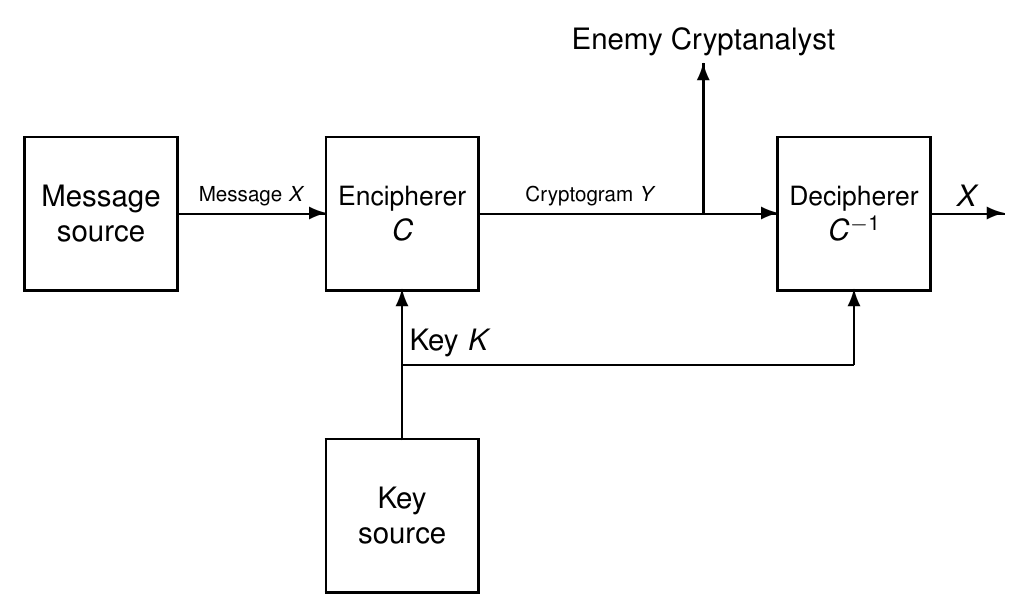
\includegraphics[scale=0.3]{images/shannon_model}
    \caption{The Shannon Encryption Model}
    \label{fig:Shannon Encryption Model}
\end{figure}
In this model, the message is a random variable with a given \textit{a priori} distribution. The key is a random variable with specified distribution, independent from the message. We need to ensure the correctness property, that is we are absolutely certain that decryption always work:
\[Pr[C_K^{-1}(C_K(X))] = 1\]
And finally, this model assumes that an adversary can get the random variable $Y  =X_K(X)$ \uline{only}. This model doesn't assume any other threat.

\subsubsection{Perfect secrecy}
Our ultimate goal is to provide \textbf{perfect secrecy}.
\begin{definition}
    Perfect secrecy means that the a posteriori distribution of the plaintext X after we know the ciphertext Y is equal to the a priori distribution of the plaintext:
    \begin{equation}
        \forall x,y\ Pr[Y=y] \neq 0 \to Pr[X=x|Y=y] = Pr[X=x]
    \end{equation}

    \textit{Equivalent definition}: Statistic independence of $X$ and $Y$

    \textit{Equivalent definition}: $H(X|Y) = H(X)$
\end{definition}

For any distribution of the plaintext, the generalized Vernam cipher provides perfect secrecy.

\evid{Influence of the Plaintext Distribution:}

\subsection{Summary and Important points}
\begin{itemize}
    \item Milestones of Prehistory: Security by obscurity, encryption with configurable secret key (Vigenère), application of the Kerckhoffs principles.
    \item Milestones of modern crypto: Kerckhoffs (1883), Shannon (1949, info-theoretical approach to crypto), Diffie-Hellman (1976, public-key crypto), DES (1977, encryption standard for non-military)
    \item Basic security properties: confidentiality, integrity, authentication
\end{itemize}



%%%%%%%%%%%%%%%%%%%%%%
%%%% Diffie Hellman%%%
%%%%%%%%%%%%%%%%%%%%%%
\section{Diffie-Hellman}
\label{sec:diffie-hellman}
\subsection{Agreement Protocol}
\label{sub:Agreement Protocol}
Assume a group generated by some \uline{public} $g$. We suppose a communication between Alice and Bob.
\begin{enumerate}
    \item Alice picks a random $x$, and compute $X = g^x$. She then sends this $X$ to Bob.
    \item Bob picks a random $y$, and computes $Y = g^y$ and the shared key $K = X^y$.
    \item Upon receiving $Y$, Alice computes $K = Y^x$.
\end{enumerate}
Thus, we have the ``shared secret'' $K = g^{xy}$. This can be defined in any group. But depending on the group, this can be easy or hard. The security requires that given $(g, g^x, g^y)$ (that are transmitted in plaintext), computing $g^{xy}$ must be hard.

This algorithms allows to set up a secret key over a public channel. Note that we still require authentication, to avoid a man-in-the-middle attack that transmits his own $g^{x'}$ and $g^{y'}$ to both parties.

The best attack is an exhaustive search on $x$. Thus, to be secured, the generated group must have a huge cardinality.
% subsection Agreement Protocol (end)

\subsection{Discrete Logarithm} % (fold)
\label{sub:Discrete Logarithm}
This problem is mentioned as such:
\begin{itemize}
    \item Parameters: $G$, a group, $g \in G$ and the $n$ the order of $g$
    \item Instance: $y$, power of $G$
    \item Problem: find $x$ such that $y = g^x$
\end{itemize}
\begin{example}
    Over $\bz_n$ this is easy (with the use of the Extended Euclidean Algorithm). Over $\bz_p^*$ or an elliptic curve, it \textbf{may} be hard
\end{example}
In a group of order $n$, the attack is easy on a quantum computer, easy if $n$ only has small prime factors. But the best algorithm for a subgroup of $\bz_p^*$ with $n$ and $p$ prime, the compelxity is
\[e^{\left(\sqrt[3]{\frac{64}{9} + o(1)}\right) (\ln n)^{\frac{1}{3}}(\ln\ln n)^{\frac{2}{3}}}\]
This is mostly precomputation, so without the need of $y$.
% subsection Discrete Logarithm (end)
\subsection{The key exchange} % (fold)
\label{sub:The key exchange}
\begin{definition}[Passive adversary]
    A \textbf{passive adversary} just listens and tries to decrypt communications (e.g. recovering the key)
\end{definition}
The Diffie-Hellman shall resist to passive attacks. Given only $g$ (public), $X$ and $Y$ (eavesdropped), it must be hard to compute $K$.

\begin{definition}[Computational Diffie-Hellman (CDH) Problem]
    \begin{itemize}
        \item Parameters: $G$ a group, $g \in G$ and $n$, the order of $G$.%
        \item Instance: $X,Y \in \langle g \rangle$
        \item Problem: find $K = g^{xy}$ where $X = g^x$ and $Y = g^y$
    \end{itemize}
\end{definition}
The hardness of this problem requires the Discrete Logarithm Problem to be hard, because CDH can be reduced to DL. This means that CDH will be \uline{at most} as hard as DL.

\subsubsection{Correct Diffie-Hellman Key Exchange} % (fold)
\label{ssub:Correct Diffie-Hellman Key Exchange}
We assume a group $\langle g \rangle$ generated by some $g$ \textcolor{red}{of prime order $q$}. At first, Alice picks $x \in \bz_q^{\textcolor{red}{*}}$, and sets $X$

\subsection{The ElGamal Public-Key Cryptosystem} % (fold)
\label{sub:The ElGamal Public-Key Cryptosystem}
\subsubsection{ElGamal Cryptosystem} % (fold)
\label{ssub:ElGamal Cryptosystem}

An important point to look at, is the \textbf{complexity} of the encryption. In subgroups of $\bz^*_p$ with $p$ of length $l$:
\begin{itemize}
    \item Domain parameter selection: $O(l^4)$
    \item Generator: $O(l^3)$
    \item Encryption: $O(l^3)$
    \item Decryption: $O(l^3)$
\end{itemize}
% subsubsection ElGamal Cryptosystem (end)
% subsection The ElGamal Public-Key Cryptosystem (end)

% subsubsection Correct Diffie-Hellman Key Exchange (end)
% subsection The key exchange (end)

\section{RSA}
\subsection{Euler and Other Chinese} % (fold)
\label{sub:Euler and Other Chinese}
\begin{theorem}[Euler Totient Function]
    Guven an integer $n$, we have the following results:
    \begin{itemize}
        \item $\forall x \in \bz_n: x \in \bz_n^* \iff \gcd(x,n) = 1$
        \item $\bz_n$ is a field $\iff \bz_n^* = \bz_n\setminus\{0\} \iff \varphi(n) = n-1 \iff n$ is prime
        \item $\forall x \in \bz_n^*$ we have $x^{\varphi(n)} \equiv 1 (\mod n)$
        \item If $e$ is such that $\gcd(e,\varphi(n)) = 1$, we let $d = e^{-1} \mod \varphi(n)$. For all $x \in \bz_n^*$, $x^d \mod n$ is the only eth root of $x$ modulo $n$
    \end{itemize}
\end{theorem}

\subsubsection{Chinese Remainder Theorem} % (fold)
\label{ssub:Chinese Remainder Theorem}
\begin{theorem}[Chinese Remainder (I)]
    Let $m$ and $n$ be two co-primes integers. For any $a,b \in \bz$, there exists $x\in\bz$ such that
    \begin{align*}
        x \equiv a\ (\mod m)\\
        x \equiv b\ (\mod n)
    \end{align*}
    And for all such solution, $x \mod (mn)$ is unique.
\end{theorem}

\begin{theorem}[Chinese Remainder (II)]
    Let $m$ and $n$ be two co-primes integers. We have
    \begin{itemize}
        \item $f: \bz_{mn} \to \bz_m \times \bz_n$ defined by $f(x) = (x \mod m, x \mod n)$ is a ring homomorphism.
        \item $f^{-1}(a,b) \equiv an(n^{-1} \mod m) + bm(m^{-1} \mod n) (\mod mn)$
    \end{itemize}
\end{theorem}
% subsubsection Chinese Remainder Theorem (end)
% subsection Euler and Other Chinese (end)
\subsection{Primality Testing} % (fold)
\label{sub:Primality Testing}

% subsection Primality Testing (end)

\subsection{RSA Basics} % (fold)
\label{sub:RSA Basics}

% subsection RSA Basics (end)

\subsection{Quadratic Residuosity} % (fold)
\label{sub:Quadratic Residuosity}

% subsection Quadratic Residuosity (end)

\subsection{The Factoring Problem} % (fold)
\label{sub:The Factoring Problem}

% subsection The Factoring Problem (end)
%%%%%%%%%%%%%%%%%%%%%
%%% APPENDIX%%%%%%%%%
%%%%%%%%%%%%%%%%%%%%%
\appendix
\section{Reminders}
\subsection{Theory Information} % (fold)
\label{sub:Theory Information}
\subsubsection{Shannon Entropy} % (fold)
\label{ssub:Shannon Entropy}
\begin{definition}[Entropy]
    We define the entropy of some string $X$ as $H(X)$. This represents the number of bits of information to represent the value of $X$. It is defined as
    \begin{equation}
        H(X) = -\somme{}{x}Pr[X=x]\log_2 Pr[X=x]
    \end{equation}
\end{definition}
 Similarly, $H(X,Y)$ is the entropy of $(X,Y)$, and $H(X|Y) = H(X,Y) - H(Y)$, that are defined, respectively, as
 \begin{align}
     H(X,Y) = -\somme{}{x}Pr[X=x, Y=y]\log_2 Pr[X=x,Y=y]\\
     H(X|Y) = -\somme{}{x}Pr[X=x,Y=y]\log_2 Pr[X=x|Y=y]
 \end{align}

 We also have the following propositions (proofs omitted):
 \begin{itemize}
     \item $H(X) \geq 0$. Equality is reached if and only if $X$ is constant.
     \item $X(X,Y) \geq H(X)$. Equality is reached if and only if $Y$ can be written as a function of $X$.
     \item $H(X,Y) \leq H(X) + H(Y)$. Equality is reached if and only if $X$ and $Y$ are independent.
     \item If $Pr[X=x] \neq 0$ for $n$ values of $x$, then $H(X) \leq \log_2 n$. Equality is reached if and only if all non-zero $Pr[X=x]$ are equal to $\frac{1}{n}$.
 \end{itemize}

 \begin{definition}[Convex]
     A real function $f$ is \textbf{convex} on $[a,b]$ if and only if
     \begin{eqnarray*}
        \forall set\ S\quad \forall t: S \to [a,b]\quad \forall p : S \to ]0,1]\\
        \somme{}{x\in S} p_x = 1 \Rightarrow \somme{}{x\in S} p_x f(t_x) \geq f\left(\somme{}{x\in S} p_x t_x\right)
     \end{eqnarray*}
 \end{definition}

% subsubsection Shannon Entropy (end)
% subsection Theory Information (end)
\subsection{Arithmetic}
We remind a few definitions and theorems that will prove useful in this chapter.
 \begin{definition}[Prime Number]
    Prime number is a positive integer which has exactly two positive factors: 1 and itself
 \end{definition}
\begin{theorem}[Unique factorization]
    Each integer n can be uniquely written
    \[n = u \times p_1^{\alpha_1} \times \cdots \times p_r^{\alpha_r}\]
    where $p_1 < \cdots < p_r$ are prime, $u = \pm 1$ and $\alpha_1,\ldots,\alpha_r$ are positive integers.
\end{theorem}
\begin{theorem}[Euclidean Division]
    For any $a \in \bz$ and any $n > 0$ there exists a unique pair $(q,r) \in \bz^2$ such that $a = qn + r$ and $0 \leq r < n$. We denote $r = a \mod n$ and have $q = \lfloor\frac{a}{n}\rfloor$
\end{theorem}
\evid{About ``mod'' notation:} $a = b \mod n$ means ``a set to (b mod n)''. on the other hand, $a \equiv b (\mod n)$ means ``a and b, once reduced modulo n, are equal''.
\subsection{Group theory}
\begin{definition}[Group]
    \label{def:group}
    An group is a set $G$ together with a mapping $G \times G \to G$ which maps $(a,b) \to a+b$ with properties:
    \begin{itemize}
        \item closure $a+b \in G$
        \item associativity $(a+b)+c = a+(b+c)$
        \item neutral element $\exists 0 : a+0 = 0+a = a$
        \item invertibility $\exists (-a) : a+(-a) = (-a)+a = a - a = 0$
    \end{itemize}
\end{definition}
\begin{definition}[Abelian group]
    \label{def:abel_group}
    An Abelian group is a group, with the additional property of commutativity
    \begin{itemize}
        \item commutativity: $a+b = b+a$
    \end{itemize}
\end{definition}
\begin{definition}[Group homomorphism]
    Given two groups $(G_1, \times_1)$ and $(G_2, \times_2)$, a mapping $f$ from $G_1$ to $G_2$ is a group homomorphism if for any $a,b \in G_1$, we have
    \begin{equation}
        f(a \times_1 b) = f(a) \times_2 f(b)
    \end{equation}
\end{definition}
\begin{example}
    If $g \in G$, the mapping $\varphi: \bz \to G$ defined by $\varphi(a) = g^a$ is a group homomorphism, because
    \[\forall a,b \in \bz,\ \varphi(a+b) = \varphi(a)\varphi(b)\]
\end{example}
\begin{theorem}[Subgroups]
    If $H$ is a subgroup of $\bz$ not reduced to $\{0\}$, then $H = n\bz$ where $n$ is the smallest positive element of $H$
\end{theorem}
\begin{definition}[Generators]
    Given a group $(G,\cdot)$, an element $g$ \textbf{generates/span} a subgroup
    \[\langle g \rangle = \{\ldots, g^{-2}, g^{-1}, g^0, g^1, g^2, \ldots\}\]
    If $\langle g \rangle$ is finite, of cardinality $n$, then $g^n = 1$ and
    \[\langle g \rangle = \{g^0,g^1,\ldots,g^{n-1}\}\]
    If $x \in \langle g \rangle,\log_g x$ is uniquely determined up to some multiple of $n$, then $\log_g x$ is an element of $\bz$ and $i \mapsto g^i$ is a group isomorphism between $\bz_n$ and $\langle g \rangle$.
\end{definition}

\begin{theorem}[Lagrange]
    In any finite group, the order of any element is a factor of the order of the group
\end{theorem}
\begin{theorem}[Generators in a group of prime order]
    If $G$ has a primer order, all elements (except 1) are generators
\end{theorem}

\subsubsection{Rings}
\begin{definition}[Rings]
    \label{def:ring}
    A ring is an Abelian group $(R,+)$ together with a mapping from $R\times R \mapsto R$ which maps $(a,b) \mapsto ab$ such that, in addition to Abelian groups properties (see definitions \ref{def:group} and \ref{def:abel_group}):
    \begin{itemize}
        \item Associativity: $(ab)c = a(bc)$
        \item neutral element: There exists 1 such that $a1 = 1a = a$
        \item Distributivity: $\forall a,b,c$, we have $a(b+c) = ab + ac$.
    \end{itemize}
\end{definition}

\begin{definition}[Commutative Ring]
    A \textbf{commutative ring} is a ring $R$ such that, in addition to Ring properties (see definition \ref{def:ring}),
    \begin{itemize}
        \item Commutativity: $\forall a,b: ab = ba$
    \end{itemize}
\end{definition}

\begin{definition}[Units]
    In a ring, not every element as an inverse for the multiplication. Thus, we denote $R^*$ the set of elements having a multiplicative inverse. Those elements are called \textbf{units}. $R*$ with the multiplication is a group ; this is \uline{the group of units of the ring $R$}
\end{definition}

\begin{definition}[Structures]
    \begin{itemize}
        \item Sub-structures:
            \begin{itemize}
                \item Subgroup: Subset of a group stable by group law and inversion
                \item ideal: Subgroup of a ring stable by multiplication by any ring element.
            \end{itemize}
        \item Spanned structure: set of all values generated by structure operations
    \end{itemize}
\end{definition}

\subsubsection{Orders in a group}
Given $x \in G$ then we have that:
\begin{itemize}
    \item $\{i \in \bz: x^i = 1\}$ is a subgroup of \bz
    \item Thus, $\{i \in \bz: x^i = 1\} = n\bz$ for some $n$ which is the smallest positive $n$ such that $x^n = 1$, which is the definition of the order.
\end{itemize}
\todo{}

\begin{example}
    The modulo 9 of big numbers of bug numbers is quite easy. As every number can be written as a sum of powers of 10 (e.g. $2\cdot 10^5 + 4\cdot 10^3 + \ldots$), every power of 10 can be reduced, modulo 9, to powers of 1. We quickly see that the reduction modulo 9 of any number can be done by adding the digits composing the number.
\end{example}

\subsection{Modular theory}

\end{document}